% the first part of the document before the begin is called preamble
\documentclass[12pt, a4paper]{article}
\usepackage{graphicx}
\graphicspath{ {./images/} }
%
\author{Leonardo Valente}
\title{Basi di Dati}

\begin{document}
    \maketitle
    \tableofcontents
    \section{Modello ER}
    Qualsiasi progetto, prima di essere mandato in produzione, segue un ciclo di vita, di solito composto da:

    \begin{itemize}
        \item Studio di fattibilità: definizione dei costi e delle priorità
        \item Raccolta di analisi e dei requisiti: studio delle proprietà del sistema
        \item Progettazione: di dati e funzioni
        \item Implementazione: ovvero la realizzazzione del progetto
        \item Validazione e collaudio: la fase di sperimentazione
        \item Funzionamento: fase di produzione
        \item Manutenzione: dove arriva il vero guadagno
    \end{itemize}

    Questo ciclo di vita segue un \textbf{modello a spirale}, quindi un ciclo dove in ogni fase è possibile
    andare avanti o indietro in base alle esigenze.

    \subsection{Progettazione}
    La progettazione delle applicazioni schematizza le operazioni sui dati e progetta il software.
    E' opportuno quindi seguire una \textbf{metodologia di progetto}.
    Essa ci permette di \textbf{suddividere} la progettazione in fasi indipenti,
    fornendo delle \textbf{strategie} da seguire e dei \textbf{criteri} di scelta.
    \\
    Nella progettazione di Database ci sono 3 fasi di progettazione: 
    \begin{itemize}
        \item Progettazione concettuale (modello ER)
        \item Progettazione logica
        \item Progettazione fisica
    \end{itemize}
    Ognuna di queste fasi si basa su un modello che permette di generare una rappresentazione
    formale (di solito uno schema) del nostro universo.
    
    \subsubsection{Progettazione concettuale}
    Traduce i requisiti del sistema in un modello ER, espresso in modo indipendente dalle scelte implementative.
    \\La descrizione si deve concentrare sui \textbf{dati} e sulle loro \textbf{relazioni}, non sulle scelte implementative.

    \subsubsection{Progettazione logica}
    Consiste nella traduzione dello schema concettuale nel modello dei dati del DBMS (Modello relazionale).

    \subsubsection{Progettazione fisica}
    Completa lo schema logico ottenuto con le specifiche proprio dell'HW/SW scelto. 
    Viene interamente effettuato dal DBMS. 
    \newpage
    \subsection{Introduzione al Modello ER}
    Il modello Entità - Relazione è un \textbf{linguaggio grafico semi-formale} per la rappresentazione di schemi concettuali.
    Esso è ormai diventato uno \textit{standard} nelle metodologie di progetto.

    Iniziamo facendo una distinzione fra \textbf{Entità} e \textbf{Relazioni}.

    \begin{itemize}
        \item \textbf{Entità}: classe di oggetti dell'applicazione di interesse con proprietà comuni e con esistenza "autonoma",
        della quale si vogliono registrare fatti specifici.
        \\Le entità hanno degli attributi che la descrivono.
        \\Una \textbf{occorrenza} (o istanza) di una entità è il singolo oggetto creato sulla base dell'entità da cui deriva
        \\Le entità vengono rappresentate nel modello ER tramite dei \textit{rettangoli}.
        \item \textbf{Attributi}: un attributo è definito su un dominio di valori.
        Esso è una funzione che associa ad ogni occorrenza \textbf{un} particolare valore (non di più!)
        Gli attributi possono essere composti e possono essere \textbf{qualsiasi cosa}.
        \\A meno che non venga definito il contrario, gli attributi sono \textbf{obbligatori}.
        \item \textbf{Relazione}: fatto che descrive un'azione o una situazione e che \textit{stabilisce legami logici tra istanze di entità}.
        \\I legami possono essere fra più di due entità e il numero delle entià coinvolte ne determina il \textbf{grado}.
        \\Ogni relazione ha un nome che la identifica.
        \\Inoltre, le relazioni possono avere degli attributi, chiamati appunto \textbf{attributi delle relazioni} che
        modellano il legame tra le entità.
        \\\\Le relazioni vengono rappresentate nel modello ER tramite dei \textit{rombi}.
        
    \end{itemize}

    \newpage
    \subsection*{Associazioni ad anello}
    Un'associazione può coinvolgere "due o più volte" la stessa entità (associazione ricorisiva o ad anello).
    \begin{figure}[htbp]
        \centering
        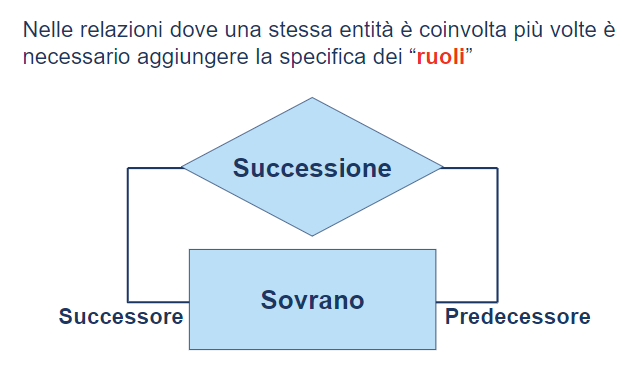
\includegraphics[scale=0.7]{roles.png}
    \end{figure}

    \section{Cardinalità delle Relazioni}
    La cardinalità delle relazioni non è altro che una coppia di valori che si associa
    a ogni entità che partecipa ad una relazione. 
    Esprimono un \textbf{limite minimo} (cardinalità minima) e un \textbf{limite massimo}
    (cardinalità massima) di istanze della \textbf{relazione R} a cui può partecipare ogni
    istanza dell'\textbf{entità E}.
    \\
    E' molto importante non sbagliare la \textit{cardinalità massima}. E' la più importante fra le due.
    Se sbagliamo la cardinalità, sbagliamo il Database!
    \\\\
    \textbf{Nota}: anche gli attributi possono avere cardinalità!
    \begin{itemize}
        \item \textbf{Molti a Molti} (3 tabelle). Quando zero o più istanze della prima entità si possono associare a zero o più istanze della seconda entità.
        \item \textbf{Uno a Molti} (2 tabelle). Quando ogni istanza della prima entità si può associare a una o più istanze della seconda entià.
        \item \textbf{Uno a Uno} (2 tabelle). Quando ogni istanza della prima entità si può associare a una e una sola istanza della seconda entià.
    \end{itemize}
    \newpage
    \subsection{Identificatori di una entità}
    E' uno strumento per l'identificazione univoca delle occorrenze di una entità.
    Ci sono due tipi di identificatori:
    \begin{itemize}
        \item \textbf{Identificatore interno} (Primary Key), che serve per distinguere in modo univoco una istanza di una entità.
        \textit{Deve essere unico}.
        \\L'identificatore interno può essere combinazione di più attributi!
        \item \textbf{Identificatore esterno} (Foreign Key), che serve per fare riferimento ad una istanza di un'altra entità avente come
        identificatore primario l'identificatore esterno dell'oggetto che stiamo prendendo in considerazione.
    \end{itemize}
    Ogni entità deve possedere almeno un identificatore (primario), ma può averne in generale più di uno (esterno).

    \section{Relazione IS-A}
    Può accadere che tra due classi rappresentate da due entità nello schema concettuale sussista la 
    \textbf{relazione IS-A}, cioè che \textbf{ogni istanza di una sia anche istanza dell'altra}.
    \\La relazione IS-A si può definire tra \textit{due entità}: \textbf{entità padre} e \textbf{entità figlio}.

    \newpage
    \subsubsection{Generalizzazione}
    Può capitare però, che l'entità padre può generalizzare diverse sottoentità rispetto ad un unico criterio. 
    In questo caso si parla di \textbf{generalizzazione}.
    \\Una generalizzazione può essere di \textit{due tipi}:
    \begin{itemize}
        \item \textbf{Completa}: l'unione delle istanze delle sottoentità è uguale all'insieme delle istanze dell'entità padre.
        \item \textbf{Non completa}.
    \end{itemize}

    \begin{figure}[htbp]
        \centering
        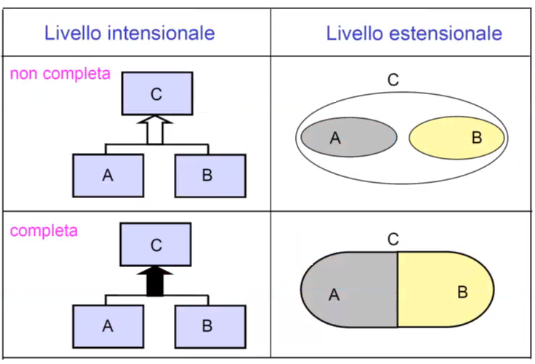
\includegraphics[scale=0.7]{generalizzazione.png}
        
        \label{<label>}
    \end{figure}

    Come possiamo vedere, nella relazione  \textit{completa}, l'unione dei due sottoinsiemi A e B è proprio 
    l'insieme "padre" C. Nella relazione \textit{NON completa}, invece, ci saranno alcuni elementi di C che non fanno
    parte ne di A e ne di B.
    \\
    Una entità può avere \textbf{al massimo una e una sola} entità padre.

    \subsubsection{Principio di ereditarietà}
    Ogni proprietà del padre è anche una proprietà del figlio, che però non viene esplicitamente riportata nello schema concettuale.
    \\L'entità figlio può avere degli attributi in più rispetto all'entità padre.



    \end{document}